% !TEX root = ../main.tex

\section{Project Status}

The status of the project is that we have completed the setup of a machine with BBR available. This involved
configuring a Linux (Ubuntu) machine with a kernel that included the BBR congestion control algorithm.

In addition, we have been able to write an experiment script in Python that collects data on BBR and CUBIC
throughput performance at varying loss rates. The network emualtor used is MahiMahi. To setup the experiment,
we use a delay shell to simulate a 100ms delay, a loss shell to control the amount of packet loss, and a link
shell to approximate a 100Mbps link.

Once the data collection is complete, the script generates a plot of the performance between BBR and CUBIC.

Our run produced the graph results in Figure~\ref{fig:rebbr8}. We can see that CUBIC only performs acceptably
when the loss rate is extremely small. At loss rates of 0.01% and above, CUBIC peformance quickly deteiriotaes.
BBR on the other hand is able to deliver decent performance when compared to CUBIC on loss rates as high as
20%.


\begin{figure}[h]
  \centering
  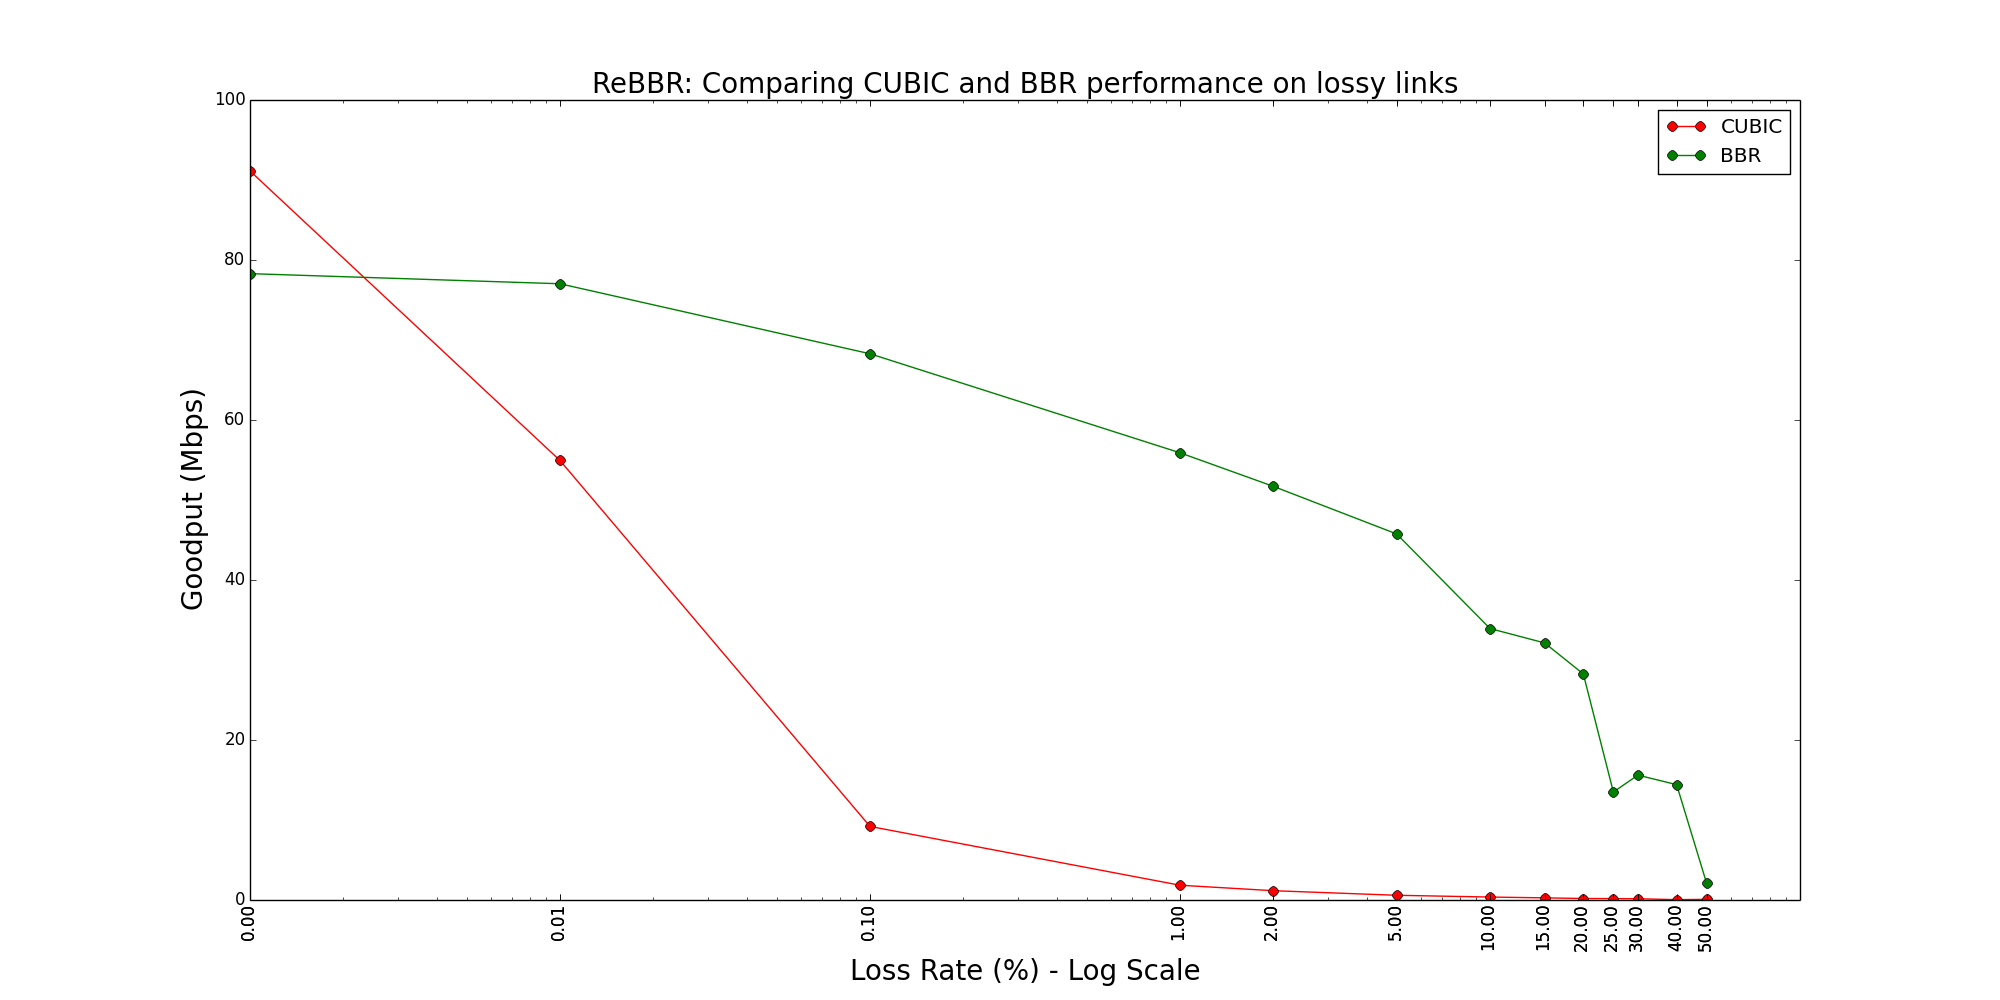
\includegraphics[height=5cm]{./img/rebbr_fig8.png}
  \caption{ReBBR: Throughput vs loss rate comparing CUBIC vs BBR.}
  \label{fig:rebbr8}
\end{figure}



\para{Plan}
For the remaining days, we need to make the experiment setup run on Google Cloud. Running a machine on Google Cloud
costs a few dollars, so for convienence and for faster iterating, we have been doing our work in a local Linux Ubuntu
VM. The next step is to replicate that setup to run successfully in the Google Cloud.

We would also like to explore how BBR compares to other modern TCP congestion control algorithms
such as VEGAS and NEW RENO.

We are also interested on evaluating how does the performance between CUBIC and BBR vary, if at all, when the network
link is running an order of magnitude slower. For example at 10Mbps, 1Mbps, 0.1Mbps (100kbps) and 0.01Mbps (10kbps).
Similarly, it would also be interesting to see the variation when the RTT changes by an order of magnitude. For example
at 0.01s, 0.1s, 1.0s, 10, 60s. Performance on the low bandwidth, high latency links should give insights into
potential benefits of BBR when deployed over slow 2G cellular links.

Finally, we need to write up our final report discussing the results we found.

Admittedly, this is  quite a bit of material and we'll try to get through as much of it as possible, time permitting.

